\chapter{Background and Threat Model}
\label{ch:background}

\section{Active Directory Architecture and Identity Primitives}
Active Directory Domain Services (AD DS) is Microsoft's distributed, hierarchical directory service that stores information about network resources and centrally manages security across Windows enterprise domains. At its foundation, Active Directory implements the Lightweight Directory Access Protocol (LDAP) to structure domain objects within a forest partition.

\subsection{Security Principals and Identifiers}
Every security entity within Active Directory—including individual users, computer accounts, security groups, and managed service accounts—is termed a \textbf{Security Principal}. Each security principal is assigned a globally unique, immutable identifier called a \textbf{Security Identifier (SID)}:
\begin{equation}
\text{SID} = \text{S-}1\text{-}5\text{-}21\text{-}D_1\text{-}D_2\text{-}D_3\text{-}R
\end{equation}
where $D_1, D_2, D_3$ denote the unique domain sub-authority, and $R$ represents the Relative Identifier (RID). RIDs below 1000 are reserved for well-known administrative entities (e.g., RID 500 represents the built-in \texttt{Administrator}, RID 512 represents \texttt{Domain Admins}, RID 519 represents \texttt{Enterprise Admins}). RIDs above 1000 designate dynamically created domain users, groups, and workstations.

\subsection{Kerberos Authentication and Token Construction}
Authentication in Active Directory is governed primarily by the Kerberos v5 protocol. The authentication workflow proceeds through the following sequential stages:
\begin{enumerate}
    \item \textbf{Authentication Service (AS) Exchange:} The client encrypts a timestamp using their hashed password and transmits an \texttt{AS-REQ} to the Key Distribution Center (KDC) running on a Domain Controller. The KDC decrypts the timestamp to verify identity and issues an \texttt{AS-REP} containing a Ticket Granting Ticket (TGT).
    \item \textbf{Privilege Attribute Certificate (PAC):} Crucially, the TGT embeds a cryptographically signed binary structure called the \textbf{Privilege Attribute Certificate (PAC)}. The PAC enumerates all security groups to which the user belongs (including transitive nested group memberships) and is signed using both the server secret and the KDC's private key.
    \item \textbf{Ticket Granting Service (TGS) Exchange:} When the client desires access to a network service (e.g., an SMB share or LDAP directory), it presents its TGT to the KDC via a \texttt{TGS-REQ}. The KDC validates the PAC signature and issues a service ticket (\texttt{TGS-REP}) encrypted with the target service's long-term key.
\end{enumerate}

When Public Key Cryptography for Initial Authentication (PKINIT) is enabled via ADCS, a client can initiate the AS exchange by presenting an X.509 digital certificate rather than a password hash. The KDC maps the certificate to a domain account using the User Principal Name (UPN) or sAMAccountName embedded within the certificate's \textbf{Subject Alternative Name (SAN)} extension, directly generating a privileged TGT.

\subsection{Access Control Lists (ACLs) and Delegation Primitives}
Every Active Directory object is protected by a \textbf{Security Descriptor} containing a Discretionary Access Control List (DACL). A DACL comprises an ordered sequence of Access Control Entries (ACEs) defining permissions granted or denied to specific SIDs. Key administrative ACEs include:
\begin{itemize}
    \item \texttt{GenericAll}: Full unrestricted control over the target object (enabling password resets, attribute modification, and object deletion).
    \item \texttt{GenericWrite}: Permission to modify any non-confidential attribute of the object.
    \item \texttt{WriteDacl}: Permission to modify the DACL itself, enabling an attacker to grant themselves \texttt{GenericAll}.
    \item \texttt{WriteOwner}: Permission to assume ownership of the object and subsequently rewrite its security descriptor.
\end{itemize}

\section{Active Directory Certificate Services (ADCS) Mechanics}
Active Directory Certificate Services (ADCS) is an integrated Windows role that allows an organization to construct an internal Public Key Infrastructure (PKI). ADCS comprises several core architectural components:

\begin{figure}[t]
    \centering
    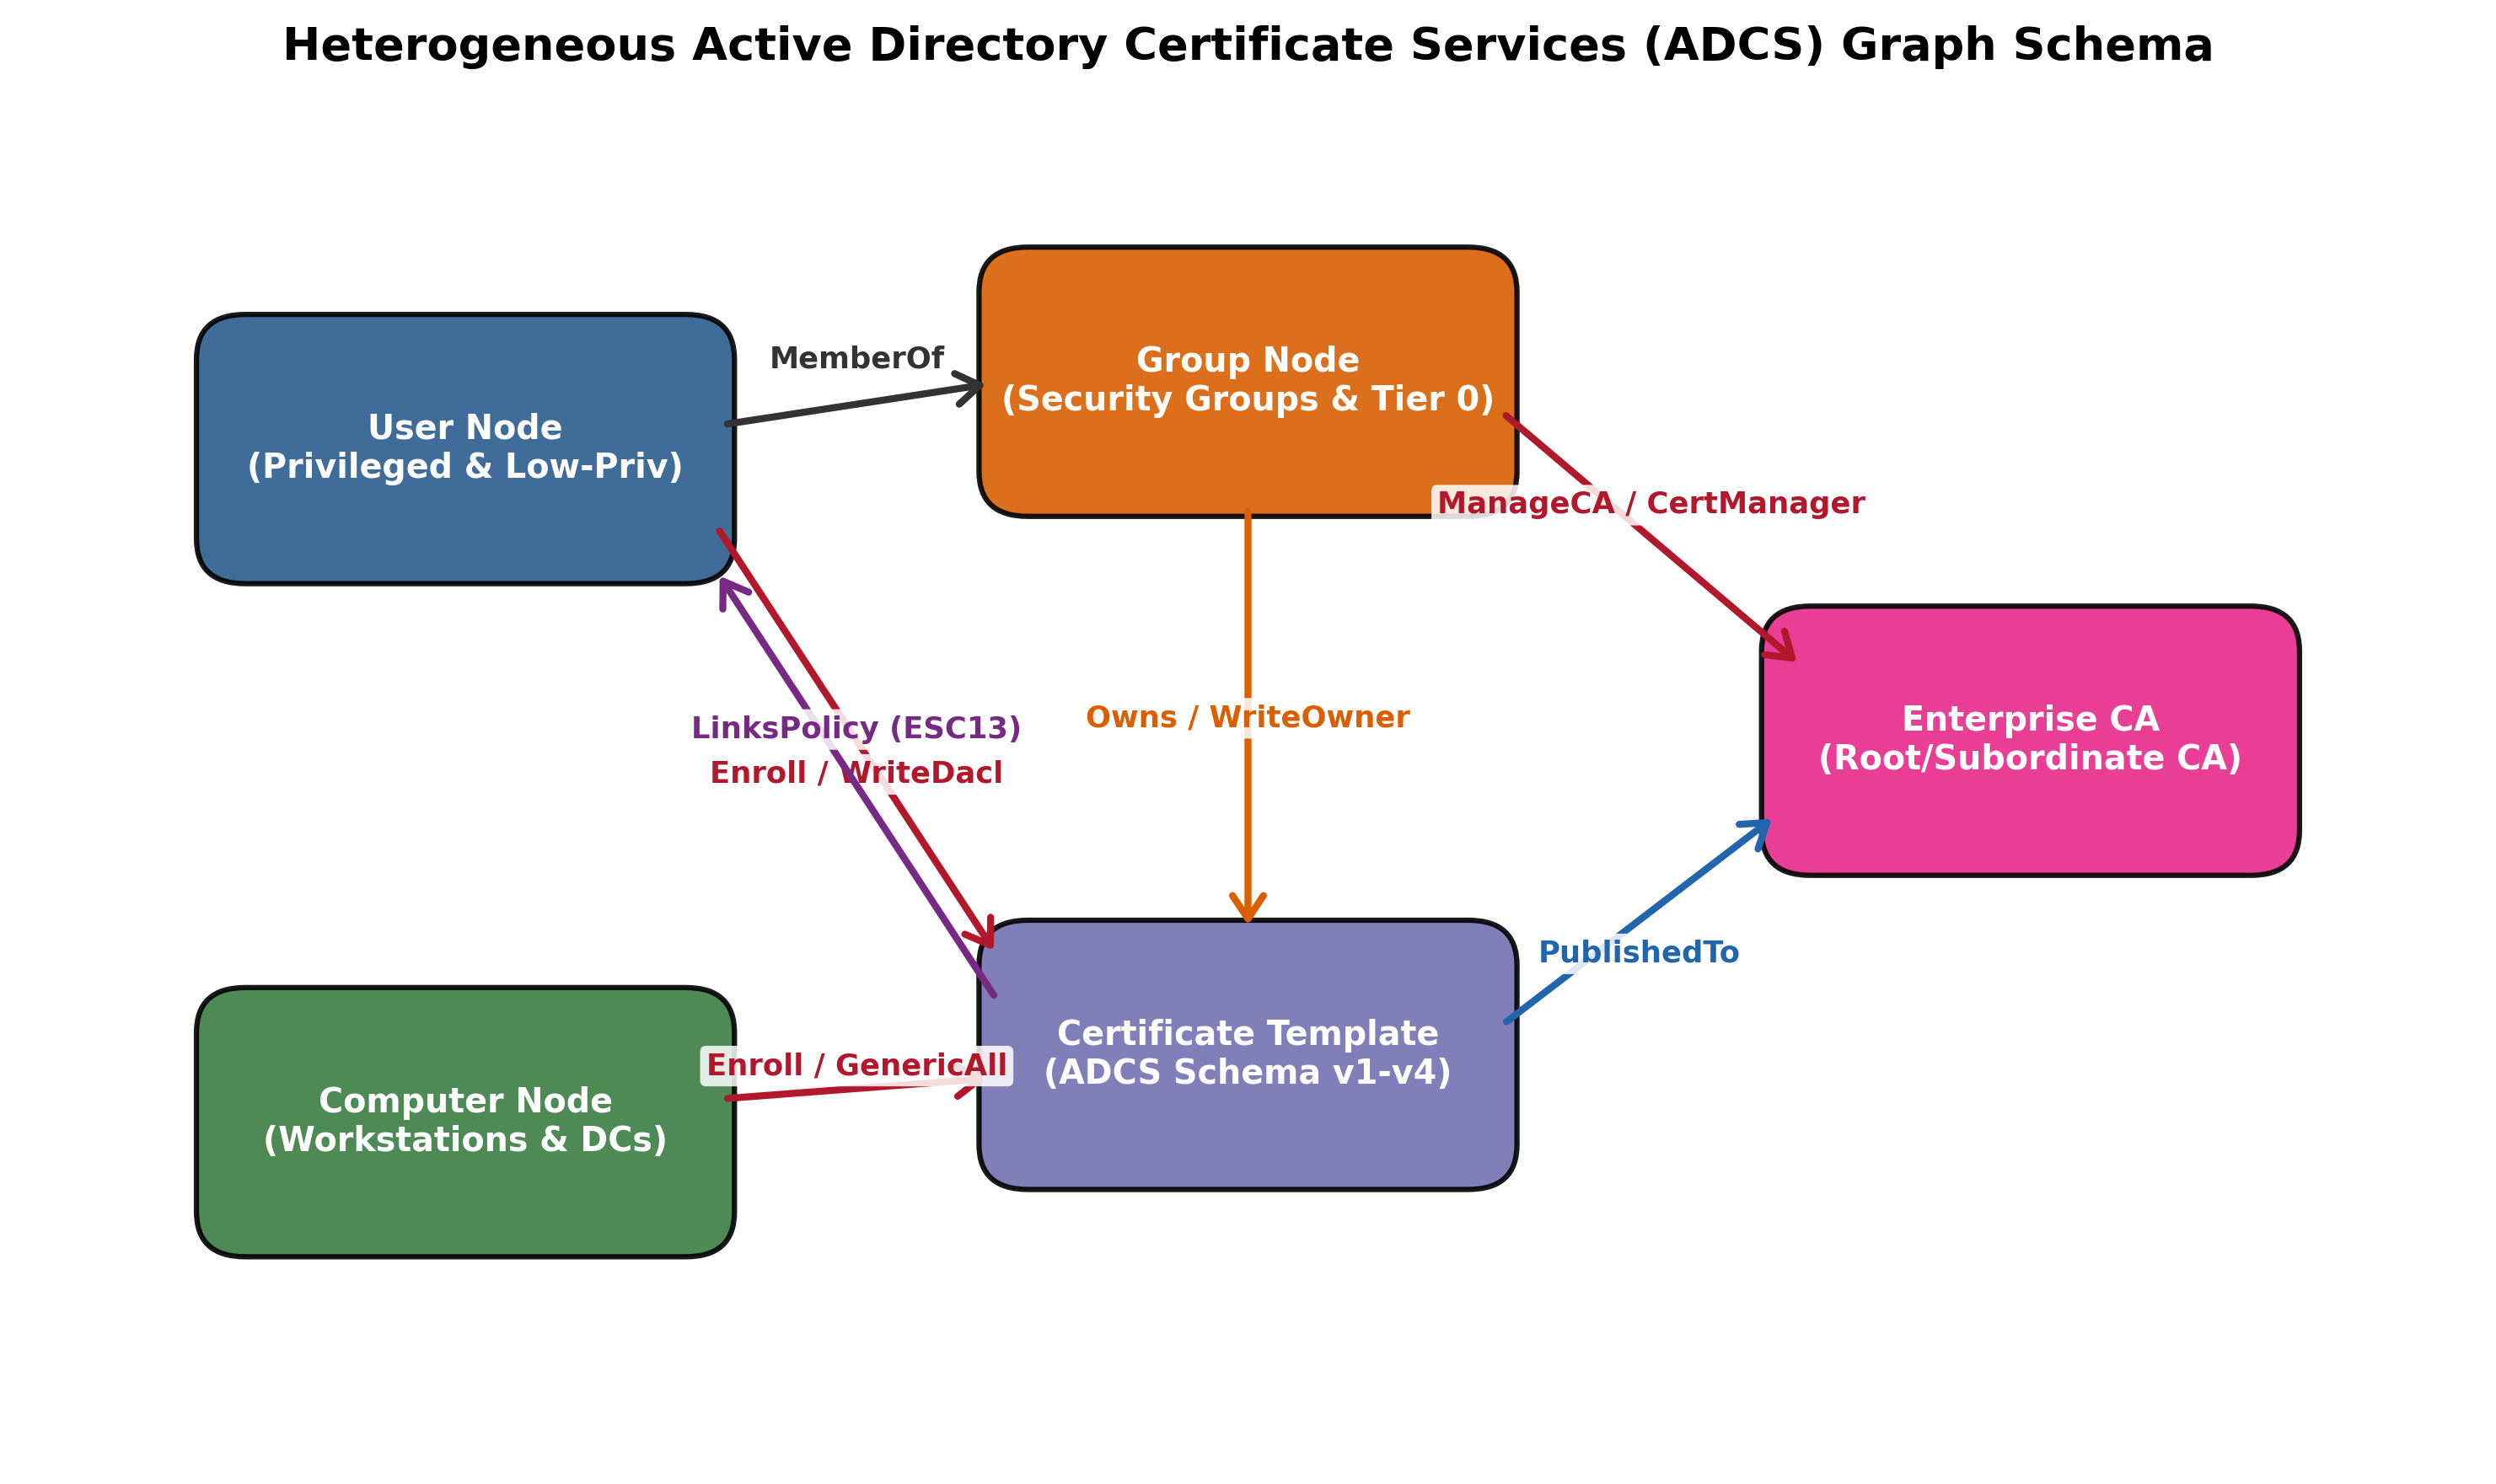
\includegraphics[width=0.85\textwidth]{figures/adcs_attack_graph_schema.png}
    \caption{Heterogeneous Active Directory Certificate Services (ADCS) Graph Schema, illustrating relations between security principals (Users, Computers, Groups), Certificate Templates, and Enterprise Certificate Authorities.}
    \label{fig:adcs_schema}
\end{figure}

\begin{enumerate}
    \item \textbf{Enterprise Certificate Authority (CA):} A server hosting the ADCS role integrated with Active Directory. Enterprise CAs store their configuration, trust anchors, and published templates directly within the LDAP Configuration partition (\texttt{CN=Configuration,DC=domain,DC=local}).
    \item \textbf{Certificate Templates:} LDAP objects (\texttt{class: pKICertificateTemplate}) defining the cryptographic and authorization parameters of certificates issued by the CA. Templates control key usage, validity periods, issuance requirements, and enrollment permissions.
    \item \textbf{Extended Key Usages (EKUs):} Object Identifiers (OIDs) embedded in certificates designating their authorized operational functions. Critical security-relevant EKUs include:
    \begin{itemize}
        \item \textbf{Client Authentication} (\texttt{1.3.6.1.5.5.7.3.2}): Authorizes the certificate for Kerberos PKINIT and TLS client authentication.
        \item \textbf{Smart Card Logon} (\texttt{1.3.6.1.4.1.311.20.2.2}): Enables interactive smart card authentication to Windows domains.
        \item \textbf{Any Purpose} (\texttt{2.5.29.37.0}): Wildcard EKU granting authorization for any cryptographic purpose.
        \item \textbf{Certificate Request Agent} (\texttt{1.3.6.1.4.1.311.20.2.1}): Authorizes an enrollee to request enrollment on behalf of other users (enrollment agent).
    \end{itemize}
    \item \textbf{Enrollment Flags and Subject Specification:} The \texttt{mspki-certificate-name-flag} attribute governs how the certificate's subject identity is populated. If the flag \texttt{CT\_FLAG\_ENROLLEE\_SUPPLIES\_SUBJECT} (\texttt{0x00000001}) is set, the certificate requestor explicitly defines the subject and SAN in their Certificate Signing Request (CSR).
\end{enumerate}

\section{Taxonomy of ADCS Vulnerability Classes (ESC1–ESC15)}
SpecterOps and subsequent security researchers categorized common ADCS misconfiguration patterns into numbered Escalation Vectors (ESC). In this research, we focus on the most impactful structural classes:

\subsection{ESC1: Enrollee Supplies Arbitrary SAN with Client Authentication}
A certificate template is vulnerable to ESC1 if all four conditions hold:
\begin{enumerate}
    \item The Enterprise CA grants enrollment rights to low-privileged users (e.g., \texttt{Authenticated Users} or \texttt{Domain Users}).
    \item The template grants enrollment permissions (\texttt{Enroll} or \texttt{ExtendedRight}) to unprivileged users.
    \item The template enables \texttt{CT\_FLAG\_ENROLLEE\_SUPPLIES\_SUBJECT}, allowing the requestor to supply an arbitrary SAN.
    \item The template specifies an EKU that permits client authentication (Client Authentication, PKINIT, Smart Card Logon, or Any Purpose).
\end{enumerate}
\textit{Exploitation Impact:} An attacker requests a certificate while supplying the UPN of a high-value administrator (e.g., \texttt{administrator@domain.local}). The CA issues a valid certificate for the administrator, which the attacker immediately exchanges for an administrative Kerberos TGT.

\subsection{ESC2: Any Purpose EKU or Missing EKU}
Similar to ESC1, but the template specifies the \texttt{Any Purpose} EKU or lacks any EKU definition altogether. Certificates without defined EKUs are treated as valid for all applications, including client authentication.

\subsection{ESC3: Certificate Request Agent (Enrollment Agent Abuse)}
The template specifies the \texttt{Certificate Request Agent} EKU without requiring manager approval. An attacker enrolls in this template to obtain an Enrollment Agent certificate, and subsequently submits a co-signed request for an administrative user against another template.

\subsection{ESC4: Vulnerable Template Access Control List (DACL)}
The template's DACL grants unprivileged users write permissions (\texttt{GenericAll}, \texttt{GenericWrite}, or \texttt{WriteDacl}).
\textit{Exploitation Impact:} The attacker overwrites the template's configuration attributes via LDAP, toggling \texttt{CT\_FLAG\_ENROLLEE\_SUPPLIES\_SUBJECT} on and adding Client Authentication to the EKU list. The attacker enrolls as Domain Admin and restores the original template parameters to conceal the compromise.

\subsection{ESC9: Missing Security Extension (No-PAC Mapping)}
Templates with schema version 2+ configured without the \texttt{szOID\_NTDS\_CA\_SECURITY\_EXT} extension (\texttt{1.3.6.1.4.1.311.25.2}), introduced in Microsoft patch KB5014754. An attacker with write access over a low-privileged account can modify its UPN to match a high-privileged account, request a certificate, and authenticate without SID validation.

\subsection{ESC13: Issuance Policy OID Linked to High-Value Groups}
Discovered by Jonas Feynman in 2023, ESC13 exploits the \texttt{msPKI-Certificate-Policy} attribute. A certificate template specifies an Issuance Policy OID that is linked via Active Directory schema to a high-value security group (e.g., Tier-0 administrators):

\begin{figure}[t]
    \centering
    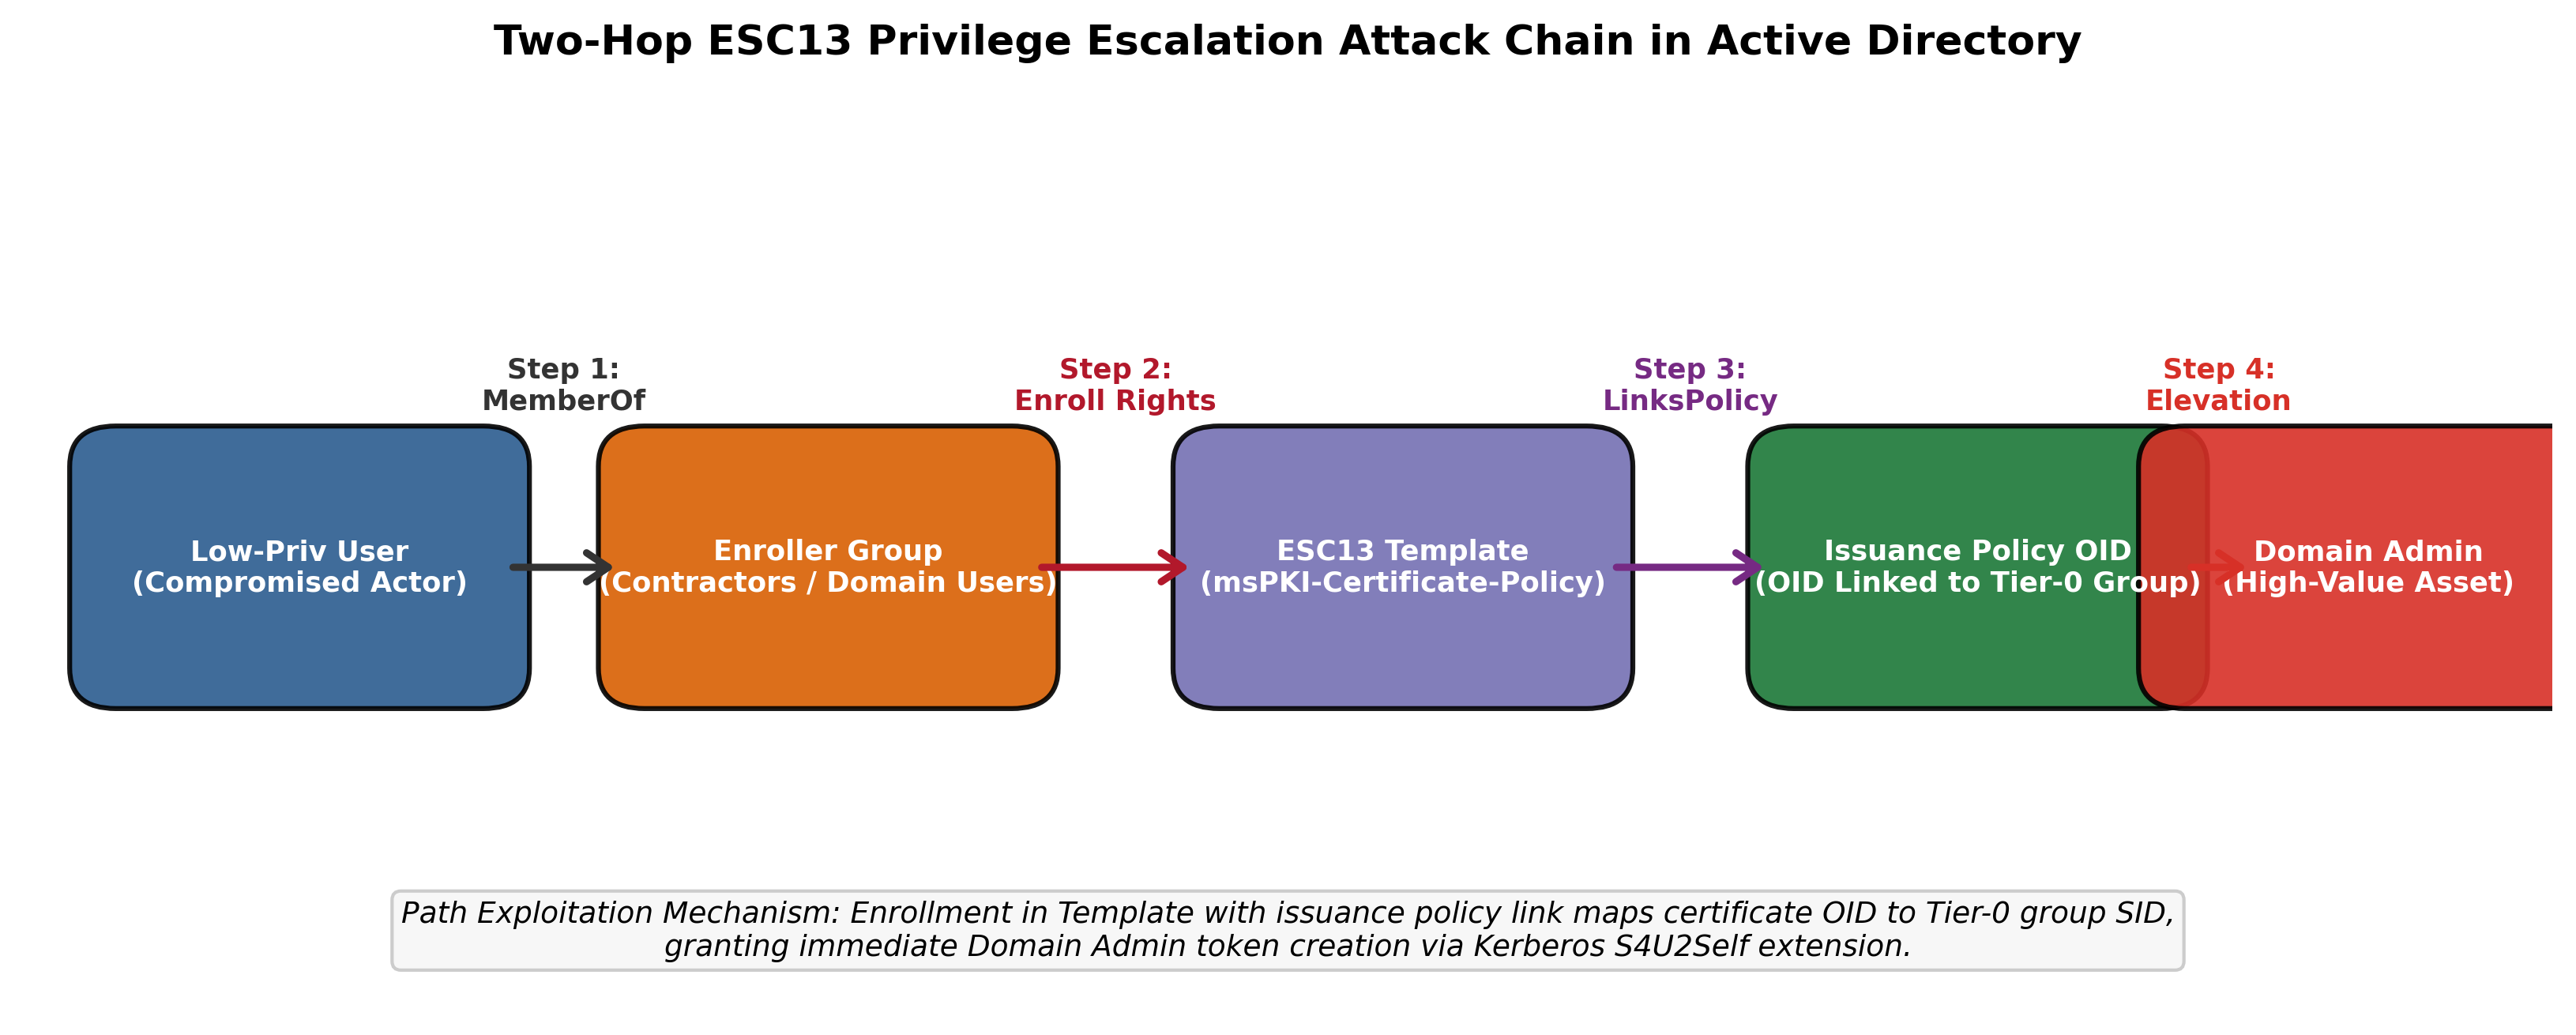
\includegraphics[width=0.95\textwidth]{figures/esc13_attack_path_diagram.png}
    \caption{Two-hop ESC13 privilege escalation attack path, showing the chain from an unprivileged user through enrollment permissions and issuance policy OID linkage to high-value domain administrative group tokens.}
    \label{fig:esc13_path}
\end{figure}

When a user enrolls in an ESC13-vulnerable template, the resulting certificate embeds the policy OID. When used for Kerberos authentication, the KDC maps the OID to the linked security group's SID and automatically appends that SID to the user's Kerberos PAC token.
\textit{Exploitation Impact:} A low-privileged user receives full Domain Admin privileges purely through cryptographic token extension.

\subsection{ESC14 and ESC15 (CVE-2024-49019 ``EKUwu'')}
ESC14 targets weak certificate mappings through \texttt{altSecurityIdentities} attribute spoofing. ESC15, disclosed in November 2024 as CVE-2024-49019, targets legacy Schema Version 1 templates. Because Schema V1 templates do not enforce application policy restrictions at the CA validation layer, an attacker can inject custom Application Policies directly into the CSR, overriding template restrictions and obtaining client authentication rights on templates intended strictly for non-authentication purposes.

\section{Formal Threat Model}
To establish rigorous scientific boundaries, we define our threat model following standard enterprise security conventions:

\subsection{Attacker Model}
\begin{enumerate}
    \item \textbf{Assumed Breach Posture:} We operate under an assumed-breach model. The adversary has already acquired unprivileged execution capability inside the internal corporate network (e.g., standard workstation access with credentials of a regular \texttt{Domain Users} account).
    \item \textbf{Telemetry and Capabilities:} The adversary has read access to the directory service via standard LDAP queries and can enumerate the active PKI infrastructure using unprivileged tools (e.g., Certipy or SharpHound).
    \item \textbf{Objective:} The adversary seeks to achieve full domain dominance (\textit{Domain Admin} or \textit{Enterprise Admin} status) by identifying and exploiting an ADCS escalation path with minimal detection risk.
\end{enumerate}

\subsection{Defender Model}
\begin{enumerate}
    \item \textbf{Auditing Scope:} The defender possesses read-only administrative auditing telemetry over the Active Directory forest, capable of extracting object attributes and DACL relationships via automated collection pipelines.
    \item \textbf{Remediation Constraints:} The defender must autonomously or semi-autonomously identify and neutralize exploitable attack paths. Crucially, the defender operates under a \textbf{business availability constraint}: defensive mitigations (such as revoking template enrollment rights or deleting groups) must not disrupt legitimate enterprise operations.
    \item \textbf{Computational Budget:} The detection architecture must execute efficiently on commodity security operations infrastructure (e.g., standard analysts' workstations with bounded RAM budgets), precluding the deployment of cumbersome full-OS virtual machine simulations for static auditing.
\end{enumerate}
